% ============================================================================================================
% Methodology section (Phase 3) -- Weather Adaptive Autonomous Driving
% Paste into the Overleaf report, or % ============================================================================================================
% Methodology section (Phase 3) -- Weather Adaptive Autonomous Driving
% Paste into the Overleaf report, or % ============================================================================================================
% Methodology section (Phase 3) -- Weather Adaptive Autonomous Driving
% Paste into the Overleaf report, or % ============================================================================================================
% Methodology section (Phase 3) -- Weather Adaptive Autonomous Driving
% Paste into the Overleaf report, or \input{methodology}. Needs the lit-review preamble plus:
%   \usepackage{algorithm}  \usepackage{algpseudocode}          (see preamble_additions.tex)
% Figure: upload ../figures/phase3/architecture.pdf (same drawing as architecture.svg on the slides).
% Citations: keys from refs_litreview.bib plus refs_methodology.bib.
% Every number is from the harness result files; see Docs/08_method_lambda_dial.md and Docs/05_results_crc_runs.md.
% ============================================================================================================
\section{Methodology}\label{sec:method}

\subsection{Baseline: per-weather conformal threshold (Phase~1)}\label{sec:method-baseline}

Our baseline is the first step of SeqCRC~\citep{andeol2025seqcrc}: conformal risk control
(CRC)~\citep{angelopoulos2024crc} on the confidence threshold of a frozen detector, with an image-level loss
$L_i(\tau)$, the fraction of ground-truth objects in calibration image~$i$ with no matched detection scoring at
least~$\tau$. Calibrated separately in each weather bin~$b$ with $n$ calibration images, the threshold is
\begin{equation}
  \hat\tau(b) \;=\; \max\Big\{\tau \;:\; \tfrac{n}{n+1}\,\hat R(\tau; b) + \tfrac{1}{n+1} \le \alpha\Big\},
  \qquad \hat R(\tau; b) = \tfrac{1}{n}\textstyle\sum_{i=1}^{n} L_i(\tau),
  \label{eq:baseline-crc}
\end{equation}
which bounds the expected miss fraction of an exchangeable test image from the same bin by~$\alpha$.
In Phase~1 we reproduced SeqCRC with its official code (the guarantee held in 5 of 5 configurations on COCO)
and ran it on DAWN~\citep{kenk2020dawn}. Our harness implements Eq.~\eqref{eq:baseline-crc} per weather bin on
YOLOv8x~\citep{ultralytics2023yolov8}. With $\alpha = 0.2$ on DAWN, the per-bin threshold keeps the held-out miss
fraction at 0.188--0.194 in every bin, at 1.6--6.2 false positives per image (FPPI), while one global threshold
misses 0.251 in fog (above $\alpha$ in 98\% of 200 splits). On BDD100K~\citep{yu2020bdd100k}, a threshold
calibrated on clear days misses 0.28--0.36 at night; per-bin thresholds restore the budget at 43--117 FPPI.

\paragraph{Limitation (the gap).} The baseline fixes the miss budget and lets the false alarms be whatever
results: at night it buys $\alpha = 0.2$ with up to 117 false alarms per image, and there is no way to ask for a
different balance. It applies one score cut to every box, it needs the weather bin at run time (our camera-only
weather estimators did not isolate fog), and its guarantee assumes exchangeable data within each bin.

\subsection{Proposed method: a calibrated trade-off dial}\label{sec:method-idea}

\textbf{Core idea.} Instead of one confidence threshold per weather bin, every detection receives a calibrated
probability $p(d)$ that it is a real object, computed from the frozen detector's own outputs, and is kept if and
only if $p(d) \ge 1/(1+\lambda)$. The single user-facing parameter $\lambda$, the number of false alarms
accepted to avoid one missed object, sets the trade-off for the use case. An F-score weight $\beta$ (and, in
Phase~4, a CRC miss budget $\alpha$) maps onto the same dial.

Table~\ref{tab:changes} lists what changes relative to the baseline. The detector, data, matching rule and
evaluation protocol stay the same; only the decision of which boxes to keep is replaced.

\begin{table}[t]
\centering\small
\caption{What our method keeps, replaces and adds relative to the Phase-1 baseline.}
\label{tab:changes}
\begin{tabularx}{\textwidth}{@{}>{\raggedright\arraybackslash}p{2.6cm}>{\raggedright\arraybackslash}X>{\raggedright\arraybackslash}X@{}}
\toprule
 & Baseline (SeqCRC step~1 per weather bin) & Ours (trade-off dial) \\
\midrule
Detector & YOLOv8x, frozen COCO weights, 1280\,px, score floor 0.001 & unchanged \\
Decision rule & one score threshold per weather bin, $s \ge \hat\tau(b)$ & per detection, $p(d) \ge 1/(1+\lambda)$; simple option: one threshold $s \ge \tau(\lambda)$ \\
Trade-off & fixed miss budget $\alpha$; false alarms unpriced & explicit input $\lambda$ (or $\beta$); $\alpha$ planned as a floor via CRC over $\lambda$ \\
Run-time inputs & score and the weather bin & score, box context and the detector's per-box outputs (no weather label) \\
Fitting & calibration half of each bin & once, on 21,831 labelled BDD100K train frames \\
Added & --- & per-box feature tap; calibrated model; $\beta \to \lambda$ map; label-free estimate of false alarms \\
\bottomrule
\end{tabularx}
\end{table}

\subsection{Architecture}\label{sec:method-arch}

Figure~\ref{fig:architecture} shows the full pipeline. Online, YOLOv8x runs once per camera frame and returns
candidate boxes $D(x)$ with class and score~$s$. We also keep the detector's per-box outputs $h(d)$ at the
anchor each box came from: the 80 class probabilities, the four distribution-focal-loss (DFL) distributions over
the box sides~\citep{li2020gfl}, the neck feature vector, and the pyramid level. A feature builder forms
$\varphi(d)$: 20 context features (score, class, size and position, rank, overlap with stronger boxes, crowding)
plus 48 per-box features (six class probabilities, strongest other class, top-two margin, sum and entropy of the
probabilities, DFL entropy per side and mean, level, and 32 principal components of the neck feature).
A gradient-boosted model maps $\varphi(d)$ to $p(d)$, and the dial keeps or drops each box. Offline, the same
frozen detector is run once over BDD100K train, boxes are labelled by matching, and the dial is fitted, checked
and then graded on data never used for fitting.

\begin{figure}[t]
  \centering
  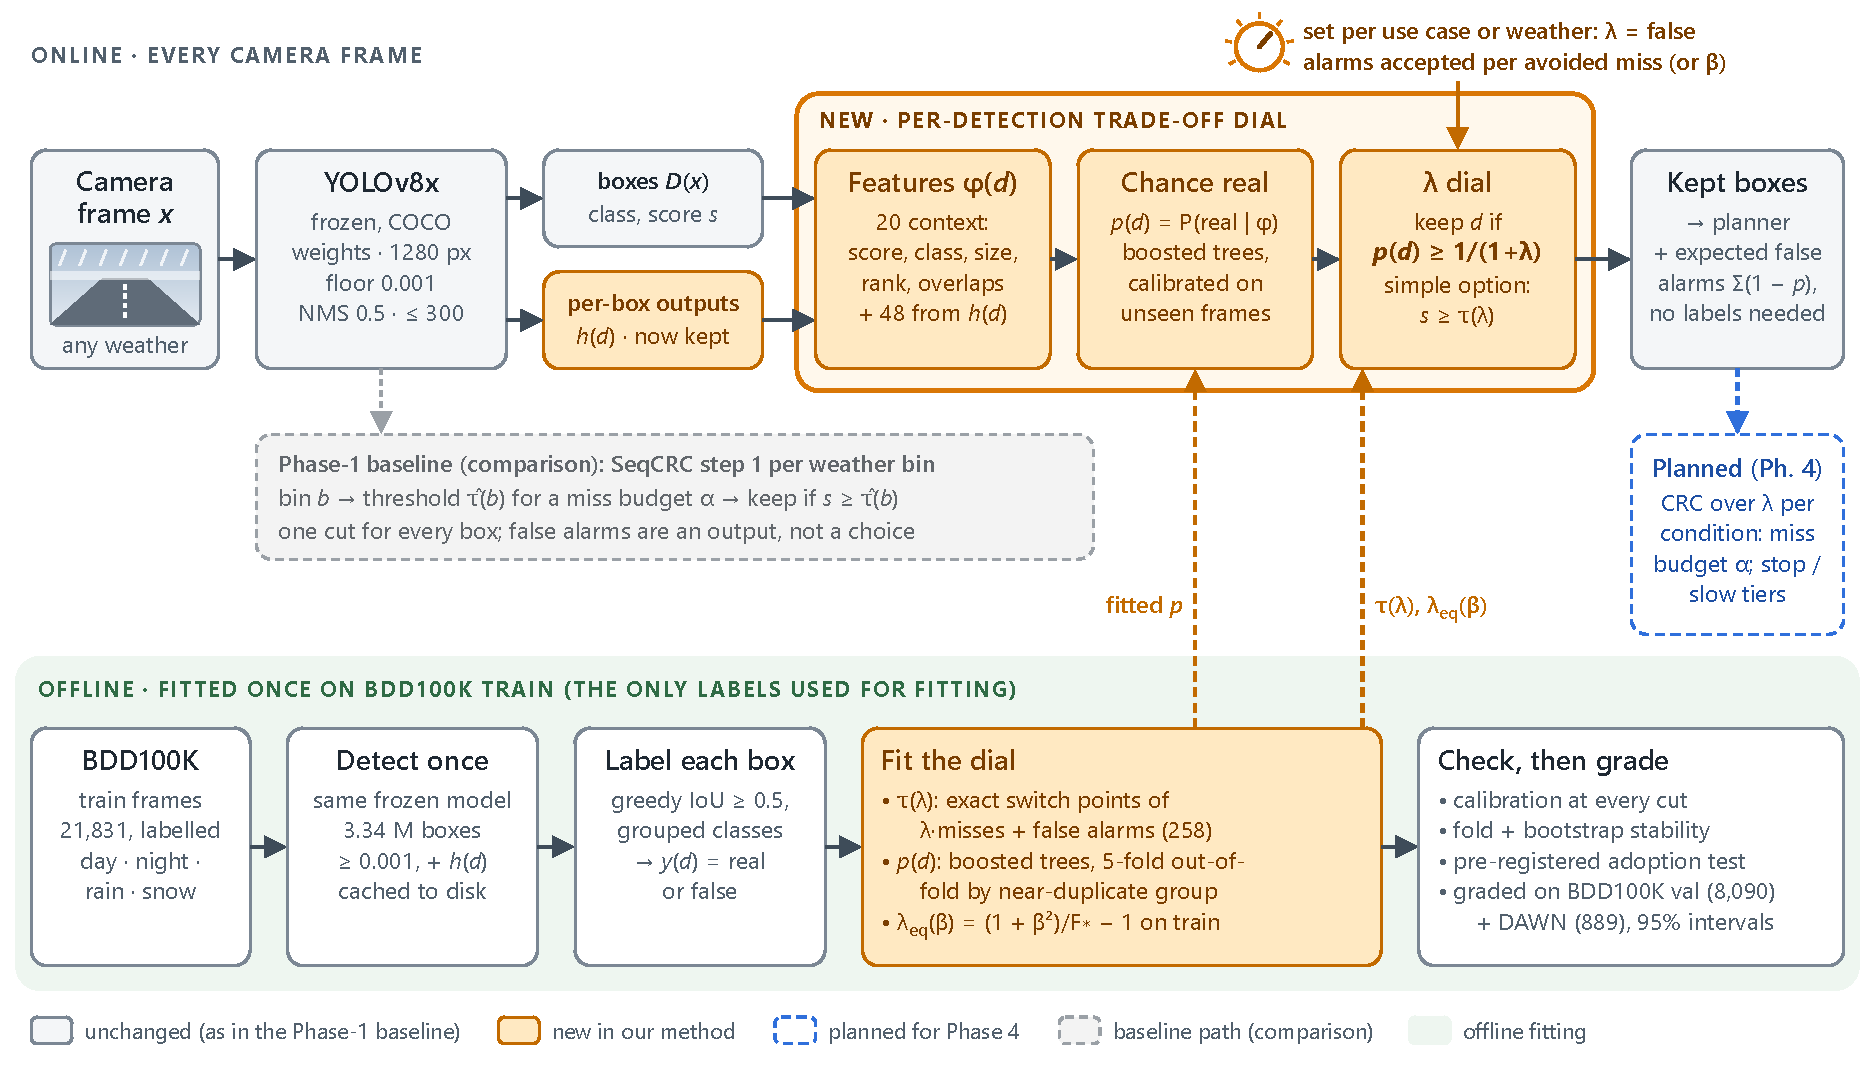
\includegraphics[width=\textwidth]{architecture}
  \caption{Architecture. New components are orange, unchanged ones grey; the dashed grey lane is the Phase-1
  baseline, kept for comparison, and the dashed blue box is planned for Phase~4. Fitting (green band) uses only
  BDD100K train; grading uses BDD100K val and DAWN.}
  \label{fig:architecture}
\end{figure}

\subsection{Algorithm}\label{sec:method-alg}

\paragraph{Cost.} For a keep rule $k$ over the detections of image $x$, let $M_k(x)$ be the number of
ground-truth objects left without a kept matched box and $F_k(x)$ the number of kept boxes that match no object.
The dial setting $\lambda > 0$ defines the cost
\begin{equation}
  C_\lambda(k) \;=\; \sum_{x}\big[\lambda\, M_k(x) + F_k(x)\big].
  \label{eq:cost}
\end{equation}

\paragraph{Option A: one threshold.} $k(d) = \mathbf{1}[s(d) \ge \tau(\lambda)]$ with
\begin{equation}
  \tau(\lambda) \;=\; \arg\min_{\tau} \sum_{x \in \mathcal{D}_{\text{train}}} \big[\lambda\, M_\tau(x) + F_\tau(x)\big].
  \label{eq:one-threshold}
\end{equation}
Greedy non-maximum suppression and greedy matching are both score-ordered, so filtering one detector run at
$\tau$ equals running the detector at $\tau$. Equation~\eqref{eq:one-threshold} is therefore solved exactly from
cumulative counts: the minimisers for all $\lambda$ are the corners of the lower convex hull of
(real kept, false kept), stored as 258 switch points.

\paragraph{Option B: per detection.} Keeping a box with probability $p$ of being real costs an expected
$1-p$ false alarms; dropping it costs an expected $\lambda p$ in misses. The cost-optimal rule is
therefore~\citep{elkan2001foundations}
\begin{equation}
  \text{keep } d \iff 1 - p(d) \le \lambda\, p(d) \iff p(d) \ge \frac{1}{1+\lambda},
  \label{eq:bayes}
\end{equation}
which is optimal when $p$ is calibrated. Because the kept set grows with $\lambda$, the miss count is
non-increasing in $\lambda$. We estimate $p(d) = \sigma\big(g(\varphi(d))\big)$ with gradient-boosted
trees~\citep{friedman2001gbm,ke2017lightgbm,pedregosa2011sklearn}. They are trained on all train detections by
minimising the log-loss
$\ell = -\sum_d \big[y_d \log p_d + (1-y_d)\log(1-p_d)\big]$, where $y_d \in \{0,1\}$ comes from greedy
IoU-$0.5$ matching with grouped classes (vehicle, two-wheeler, person). We check calibration with the expected
calibration error~\citep{guo2017calibration} and with the share of real boxes among detections near each cut
$1/(1+\lambda)$.

\paragraph{F-score units.} With calibrated probabilities, the $F_\beta$-optimal cut is $F^*_\beta/(1+\beta^2)$,
where $F^*_\beta$ is the best achievable $F_\beta$~\citep{zhao2013beyond,lipton2014optimal}. Setting this cut
equal to $1/(1+\lambda)$ gives the equivalent dial setting
\begin{equation}
  \lambda_{\text{eq}}(\beta) \;=\; \frac{1+\beta^2}{F^*_\beta} - 1,
  \label{eq:fbeta}
\end{equation}
with $F^*_\beta$ measured on train for each option. For example, $F_1$ corresponds to $\lambda \approx 1.8$ and
$F_2$ to $\lambda \approx 6.2$ with the per-detection option.

\paragraph{Planned: a miss budget on top of the dial (CRC over $\lambda$).} Because the image-level miss fraction
$L_i(\lambda)$ is non-increasing in $\lambda$, the baseline's rule~\eqref{eq:baseline-crc} applies to $\lambda$
itself. Per condition $c$ with $n_c$ calibration images,
\begin{equation}
  \hat\lambda_c \;=\; \inf\Big\{\lambda \;:\; \tfrac{n_c}{n_c+1}\,\hat R_c(\lambda) + \tfrac{1}{n_c+1} \le \alpha\Big\},
  \label{eq:crc-lambda}
\end{equation}
and deploying $\max(\lambda_{\text{user}}, \hat\lambda_c)$ keeps the CRC guarantee
$\mathbb{E}[L_{\text{test}}] \le \alpha$ under exchangeability within the condition, while never being less
cautious than the user asked. The fit is infeasible when $\alpha$ is below the miss fraction at the score floor
(11--18\% of objects are never detected).

\begin{algorithm}[t]
\caption{Fitting the dial (offline, BDD100K train only)}\label{alg:fit}
\begin{algorithmic}[1]
\Require labelled train frames $\mathcal{D}_{\text{train}}$; frozen detector $f$
\ForAll{$x \in \mathcal{D}_{\text{train}}$}
  \State $(D(x), h) \gets f(x)$ \Comment{floor 0.001, NMS 0.5, $\le 300$ boxes; keep per-box outputs}
  \State $y(d) \gets$ greedy IoU $\ge 0.5$ match of $d \in D(x)$ to labels \Comment{grouped classes}
\EndFor
\State \textbf{Option A:} sort scores; keep ends of equal-score blocks; cumulative real and false counts
\State \hspace{1.2em} $\tau(\cdot) \gets$ corners of the lower convex hull \Comment{all $\lambda$ at once}
\State \textbf{Option B:} $\varphi(d) \gets [\text{context}(d, D(x)),\ \text{per-box}(h(d))]$ \Comment{PCA fitted on train}
\State \hspace{1.2em} $g \gets$ gradient boosting on $\{(\varphi(d), y(d))\}$ \Comment{log-loss}
\State \hspace{1.2em} $p_{\text{oof}} \gets$ 5-fold out-of-fold probabilities, folds by near-duplicate group
\ForAll{$\beta$}
  \State $\lambda_{\text{eq}}(\beta) \gets (1+\beta^2)/F^*_\beta - 1$ \Comment{F-score map, $F^*_\beta$ on train}
\EndFor
\State check calibration near every cut $1/(1+\lambda)$ and fold stability; adopt only if the pre-registered criteria hold
\State \Return $\tau(\cdot)$, $g$ (with PCA), $\lambda_{\text{eq}}(\cdot)$
\end{algorithmic}
\end{algorithm}

\begin{algorithm}[t]
\caption{Applying the dial (online, every camera frame)}\label{alg:deploy}
\begin{algorithmic}[1]
\Require frame $x$; setting $\lambda$ (or $\beta$); option $\in\{$A, B$\}$
\If{$\beta$ is given} \State $\lambda \gets \lambda_{\text{eq}}(\beta)$ \Comment{F-score map} \EndIf
\If{a budget $\alpha$ is certified for condition $c$} \State $\lambda \gets \max(\lambda, \hat\lambda_c)$ \Comment{planned: CRC over $\lambda$} \EndIf
\State $(D, h) \gets f(x)$ \Comment{one detector pass}
\ForAll{$d \in D$}
  \If{option A}
    \State keep $d$ iff $s(d) \ge \tau(\lambda)$
  \Else
    \State $p(d) \gets \sigma(g(\varphi(d)))$; keep $d$ iff $p(d) \ge 1/(1+\lambda)$ \Comment{cost-optimal cut}
  \EndIf
\EndFor
\State $\widehat{\mathrm{FA}} \gets \sum_{d \text{ kept}} (1 - p(d))$ \Comment{expected false alarms, no labels needed}
\State \Return kept detections, $\widehat{\mathrm{FA}}$
\end{algorithmic}
\end{algorithm}

\subsection{Design choices}\label{sec:method-design}

Table~\ref{tab:design} gives each design choice, the reason for it, and the alternatives we tried or
considered. Most of the alternatives were run in the harness, several under pre-registered criteria.

\begin{table}[t]
\centering\small
\caption{Design choices, the reasons for them, and the alternatives considered (with the evidence).}
\label{tab:design}
\begin{tabularx}{\textwidth}{@{}>{\raggedright\arraybackslash}p{2.9cm}>{\raggedright\arraybackslash}X>{\raggedright\arraybackslash}X@{}}
\toprule
Choice & Why & Alternatives considered \\
\midrule
Keep the detector frozen; decide after it &
calibration stays valid; one detector run serves every setting; no retraining per condition &
domain adaptation (DA-Detect: 20.41 vs 21.44 AP@50 on real DAWN fog in Phase~1); fine-tuning (invalidates every calibration) \\
Trade-off as $\lambda$, false alarms per avoided miss &
use case sets the balance; the optimal rule is explicit (Eq.~\ref{eq:bayes}); $\beta$ and $\alpha$ map onto it &
fixed $\alpha$ only (baseline, false alarms unpriced); maximise $F_1$ (one fixed balance); FPPI cap \\
Decide per detection &
87--91\% of a per-image oracle's advantage on BDD100K is chance; the learnable signal is in individual boxes &
per-image thresholds from pixels, from the confidence profile, or from YOLOv8x image features (all failed pre-registered tests); box-combination rules; summed-confidence maps \\
One threshold kept as the simple option &
one auditable number per $\lambda$; per-weather thresholds give no gain (0.98--1.03$\times$ the cost) &
per-weather thresholds (the baseline's form) \\
Gradient-boosted trees on detector outputs &
tabular inputs; trains in minutes on CPU; calibrated without post-hoc scaling (expected calibration error 0.11 points on BDD100K val) &
recalibrating the score alone (this is Option~A); a neural head; retraining YOLOv8x's head \\
YOLOv8x's own per-box outputs as features &
pre-registered gain: cost 0.972$\times$ (0.969--0.975) of the context-only model on BDD100K, not worse on DAWN (0.995) &
context features only (model~1); a separate CNN on box crops (more compute) \\
One model for every $\beta$ &
theory: only the cut moves with $\beta$; dedicated $\beta$-weighted models tie (0.997--1.001$\times$) &
one cost-weighted model per $\beta$ \\
Fit on BDD100K train; grade on BDD100K val and DAWN &
nothing is chosen on graded data; DAWN tests transfer to real fog, rain, sand and snow &
calibrating on halves of the test pool (the baseline protocol) \\
Grouped classes in matching &
car/truck confusions are not safety misses &
class-aware matching (run~1) \\
\bottomrule
\end{tabularx}
\end{table}

\subsection{Experiment plan (Phase~4)}\label{sec:method-plan}

\paragraph{Data and splits.} The dial is fitted on 21,831 BDD100K train frames (3.34\,M detections), with 5-fold
out-of-fold estimates grouped by near-duplicate group. It is graded on BDD100K val (8,090 frames in seven
weather-by-time bins) and on DAWN (889 frames with clean labels: fog 256, rain 187, sand 243, snow 203).
Neither set is used for any choice. For CRC over $\lambda$ we use 200 random calibration/test halves per
condition, keeping near-duplicate groups together, as in the baseline runs.

\paragraph{Metrics.} The main metric is the cost $C_\lambda$ relative to one threshold, with 95\% image-bootstrap
intervals~\citep{efron1993bootstrap}. We also report recall, precision and false alarms per image at
$\lambda \in \{1, 3, 10, 30, 100\}$; $F_\beta$ at $\beta \in \{0.5, 1, 2\}$ against no tuning and the best
in-sample constant; and calibration (expected calibration error, share real near each cut). For CRC over
$\lambda$ we report the held-out miss fraction against $\alpha$ (share of splits above), its price in false alarms
per image, and the smallest certifiable $\alpha$.

\paragraph{Baselines.} (i) No tuning ($\tau = 0.25$, the Ultralytics default). (ii) One global CRC threshold.
(iii) The per-weather CRC threshold, Eq.~\eqref{eq:baseline-crc} (Phase-1 baseline). (iv) Option~A, the one-threshold
dial. (v) The context-only per-detection model. As reference bounds that no deployable rule can reach, we also
report the best constant threshold chosen in-sample per condition and the per-frame hindsight best.

\paragraph{Ablations.} (a) Retraining without each feature group: class probabilities, neck components, DFL
entropy, level, context. (b) Per-condition recalibration, which targets the under-stated probabilities in DAWN fog
(17\% real at the 9.1\% cut). (c) Training-set size: 25, 50 and 100\% of frames. (d) Detector size and input
resolution: YOLOv8x at 640 versus 1280, and YOLOv8s. (e) CRC over $\lambda$ versus CRC over $\tau$ at equal
$\alpha$. Already completed: model~1 versus model~2, per-weather thresholds, and dedicated $\beta$ models.

\paragraph{Compute.} Measured on our laptop GPU (RTX 3050 Ti, 4\,GB):
\begin{itemize}
  \item YOLOv8x at 1280\,px takes 0.15--0.17\,s per frame;
  \item extracting per-box outputs for all 30.9k frames takes about 85 minutes;
  \item fitting the per-detection model takes about 11 minutes on the CPU;
  \item the CRC splits take minutes on the CPU.
\end{itemize}
We will use an NRP A100 for the new detector passes in ablation~(d) and for the repeated fits in (a)--(c).
At an estimated $\ge 10\times$ the laptop's throughput, these take a few GPU-hours in total. The laptop
remains a fallback for every step.
. Needs the lit-review preamble plus:
%   \usepackage{algorithm}  \usepackage{algpseudocode}          (see preamble_additions.tex)
% Figure: upload ../figures/phase3/architecture.pdf (same drawing as architecture.svg on the slides).
% Citations: keys from refs_litreview.bib plus refs_methodology.bib.
% Every number is from the harness result files; see Docs/08_method_lambda_dial.md and Docs/05_results_crc_runs.md.
% ============================================================================================================
\section{Methodology}\label{sec:method}

\subsection{Baseline: per-weather conformal threshold (Phase~1)}\label{sec:method-baseline}

Our baseline is the first step of SeqCRC~\citep{andeol2025seqcrc}: conformal risk control
(CRC)~\citep{angelopoulos2024crc} on the confidence threshold of a frozen detector, with an image-level loss
$L_i(\tau)$, the fraction of ground-truth objects in calibration image~$i$ with no matched detection scoring at
least~$\tau$. Calibrated separately in each weather bin~$b$ with $n$ calibration images, the threshold is
\begin{equation}
  \hat\tau(b) \;=\; \max\Big\{\tau \;:\; \tfrac{n}{n+1}\,\hat R(\tau; b) + \tfrac{1}{n+1} \le \alpha\Big\},
  \qquad \hat R(\tau; b) = \tfrac{1}{n}\textstyle\sum_{i=1}^{n} L_i(\tau),
  \label{eq:baseline-crc}
\end{equation}
which bounds the expected miss fraction of an exchangeable test image from the same bin by~$\alpha$.
In Phase~1 we reproduced SeqCRC with its official code (the guarantee held in 5 of 5 configurations on COCO)
and ran it on DAWN~\citep{kenk2020dawn}. Our harness implements Eq.~\eqref{eq:baseline-crc} per weather bin on
YOLOv8x~\citep{ultralytics2023yolov8}. With $\alpha = 0.2$ on DAWN, the per-bin threshold keeps the held-out miss
fraction at 0.188--0.194 in every bin, at 1.6--6.2 false positives per image (FPPI), while one global threshold
misses 0.251 in fog (above $\alpha$ in 98\% of 200 splits). On BDD100K~\citep{yu2020bdd100k}, a threshold
calibrated on clear days misses 0.28--0.36 at night; per-bin thresholds restore the budget at 43--117 FPPI.

\paragraph{Limitation (the gap).} The baseline fixes the miss budget and lets the false alarms be whatever
results: at night it buys $\alpha = 0.2$ with up to 117 false alarms per image, and there is no way to ask for a
different balance. It applies one score cut to every box, it needs the weather bin at run time (our camera-only
weather estimators did not isolate fog), and its guarantee assumes exchangeable data within each bin.

\subsection{Proposed method: a calibrated trade-off dial}\label{sec:method-idea}

\textbf{Core idea.} Instead of one confidence threshold per weather bin, every detection receives a calibrated
probability $p(d)$ that it is a real object, computed from the frozen detector's own outputs, and is kept if and
only if $p(d) \ge 1/(1+\lambda)$. The single user-facing parameter $\lambda$, the number of false alarms
accepted to avoid one missed object, sets the trade-off for the use case. An F-score weight $\beta$ (and, in
Phase~4, a CRC miss budget $\alpha$) maps onto the same dial.

Table~\ref{tab:changes} lists what changes relative to the baseline. The detector, data, matching rule and
evaluation protocol stay the same; only the decision of which boxes to keep is replaced.

\begin{table}[t]
\centering\small
\caption{What our method keeps, replaces and adds relative to the Phase-1 baseline.}
\label{tab:changes}
\begin{tabularx}{\textwidth}{@{}>{\raggedright\arraybackslash}p{2.6cm}>{\raggedright\arraybackslash}X>{\raggedright\arraybackslash}X@{}}
\toprule
 & Baseline (SeqCRC step~1 per weather bin) & Ours (trade-off dial) \\
\midrule
Detector & YOLOv8x, frozen COCO weights, 1280\,px, score floor 0.001 & unchanged \\
Decision rule & one score threshold per weather bin, $s \ge \hat\tau(b)$ & per detection, $p(d) \ge 1/(1+\lambda)$; simple option: one threshold $s \ge \tau(\lambda)$ \\
Trade-off & fixed miss budget $\alpha$; false alarms unpriced & explicit input $\lambda$ (or $\beta$); $\alpha$ planned as a floor via CRC over $\lambda$ \\
Run-time inputs & score and the weather bin & score, box context and the detector's per-box outputs (no weather label) \\
Fitting & calibration half of each bin & once, on 21,831 labelled BDD100K train frames \\
Added & --- & per-box feature tap; calibrated model; $\beta \to \lambda$ map; label-free estimate of false alarms \\
\bottomrule
\end{tabularx}
\end{table}

\subsection{Architecture}\label{sec:method-arch}

Figure~\ref{fig:architecture} shows the full pipeline. Online, YOLOv8x runs once per camera frame and returns
candidate boxes $D(x)$ with class and score~$s$. We also keep the detector's per-box outputs $h(d)$ at the
anchor each box came from: the 80 class probabilities, the four distribution-focal-loss (DFL) distributions over
the box sides~\citep{li2020gfl}, the neck feature vector, and the pyramid level. A feature builder forms
$\varphi(d)$: 20 context features (score, class, size and position, rank, overlap with stronger boxes, crowding)
plus 48 per-box features (six class probabilities, strongest other class, top-two margin, sum and entropy of the
probabilities, DFL entropy per side and mean, level, and 32 principal components of the neck feature).
A gradient-boosted model maps $\varphi(d)$ to $p(d)$, and the dial keeps or drops each box. Offline, the same
frozen detector is run once over BDD100K train, boxes are labelled by matching, and the dial is fitted, checked
and then graded on data never used for fitting.

\begin{figure}[t]
  \centering
  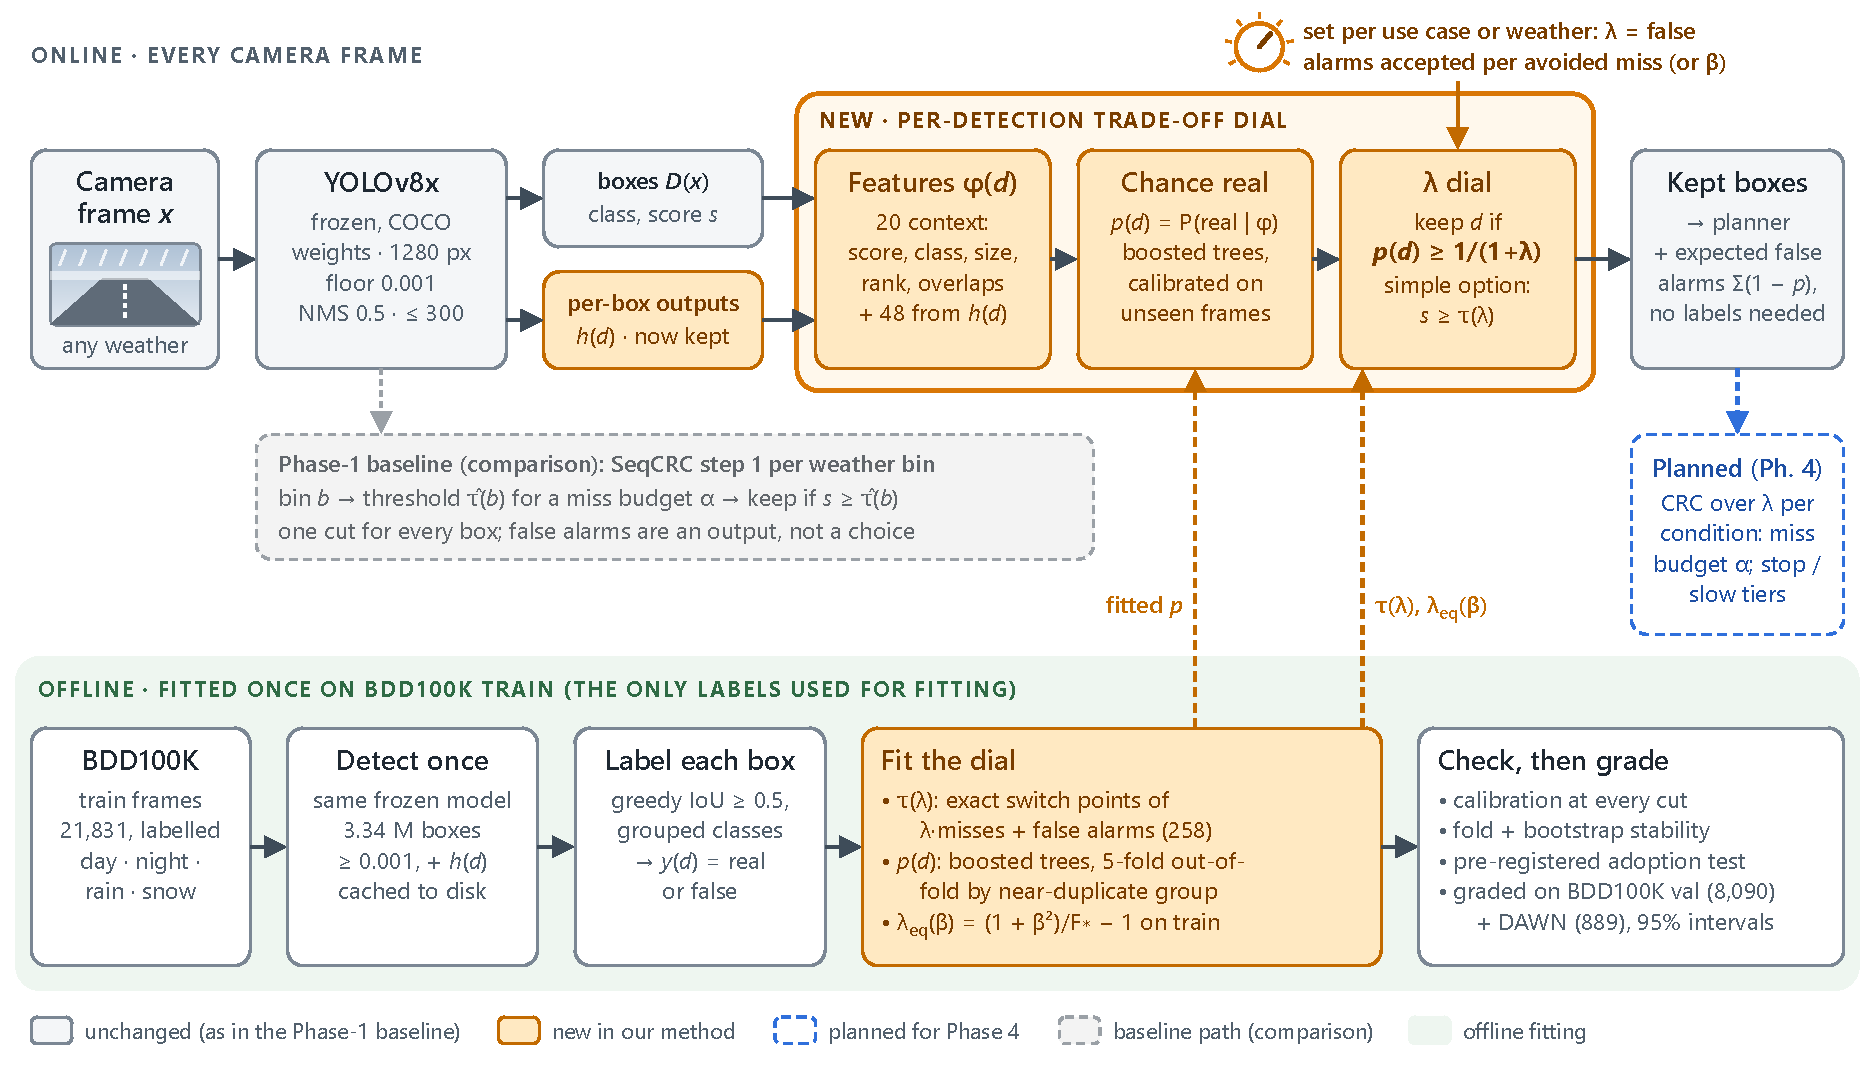
\includegraphics[width=\textwidth]{architecture}
  \caption{Architecture. New components are orange, unchanged ones grey; the dashed grey lane is the Phase-1
  baseline, kept for comparison, and the dashed blue box is planned for Phase~4. Fitting (green band) uses only
  BDD100K train; grading uses BDD100K val and DAWN.}
  \label{fig:architecture}
\end{figure}

\subsection{Algorithm}\label{sec:method-alg}

\paragraph{Cost.} For a keep rule $k$ over the detections of image $x$, let $M_k(x)$ be the number of
ground-truth objects left without a kept matched box and $F_k(x)$ the number of kept boxes that match no object.
The dial setting $\lambda > 0$ defines the cost
\begin{equation}
  C_\lambda(k) \;=\; \sum_{x}\big[\lambda\, M_k(x) + F_k(x)\big].
  \label{eq:cost}
\end{equation}

\paragraph{Option A: one threshold.} $k(d) = \mathbf{1}[s(d) \ge \tau(\lambda)]$ with
\begin{equation}
  \tau(\lambda) \;=\; \arg\min_{\tau} \sum_{x \in \mathcal{D}_{\text{train}}} \big[\lambda\, M_\tau(x) + F_\tau(x)\big].
  \label{eq:one-threshold}
\end{equation}
Greedy non-maximum suppression and greedy matching are both score-ordered, so filtering one detector run at
$\tau$ equals running the detector at $\tau$. Equation~\eqref{eq:one-threshold} is therefore solved exactly from
cumulative counts: the minimisers for all $\lambda$ are the corners of the lower convex hull of
(real kept, false kept), stored as 258 switch points.

\paragraph{Option B: per detection.} Keeping a box with probability $p$ of being real costs an expected
$1-p$ false alarms; dropping it costs an expected $\lambda p$ in misses. The cost-optimal rule is
therefore~\citep{elkan2001foundations}
\begin{equation}
  \text{keep } d \iff 1 - p(d) \le \lambda\, p(d) \iff p(d) \ge \frac{1}{1+\lambda},
  \label{eq:bayes}
\end{equation}
which is optimal when $p$ is calibrated. Because the kept set grows with $\lambda$, the miss count is
non-increasing in $\lambda$. We estimate $p(d) = \sigma\big(g(\varphi(d))\big)$ with gradient-boosted
trees~\citep{friedman2001gbm,ke2017lightgbm,pedregosa2011sklearn}. They are trained on all train detections by
minimising the log-loss
$\ell = -\sum_d \big[y_d \log p_d + (1-y_d)\log(1-p_d)\big]$, where $y_d \in \{0,1\}$ comes from greedy
IoU-$0.5$ matching with grouped classes (vehicle, two-wheeler, person). We check calibration with the expected
calibration error~\citep{guo2017calibration} and with the share of real boxes among detections near each cut
$1/(1+\lambda)$.

\paragraph{F-score units.} With calibrated probabilities, the $F_\beta$-optimal cut is $F^*_\beta/(1+\beta^2)$,
where $F^*_\beta$ is the best achievable $F_\beta$~\citep{zhao2013beyond,lipton2014optimal}. Setting this cut
equal to $1/(1+\lambda)$ gives the equivalent dial setting
\begin{equation}
  \lambda_{\text{eq}}(\beta) \;=\; \frac{1+\beta^2}{F^*_\beta} - 1,
  \label{eq:fbeta}
\end{equation}
with $F^*_\beta$ measured on train for each option. For example, $F_1$ corresponds to $\lambda \approx 1.8$ and
$F_2$ to $\lambda \approx 6.2$ with the per-detection option.

\paragraph{Planned: a miss budget on top of the dial (CRC over $\lambda$).} Because the image-level miss fraction
$L_i(\lambda)$ is non-increasing in $\lambda$, the baseline's rule~\eqref{eq:baseline-crc} applies to $\lambda$
itself. Per condition $c$ with $n_c$ calibration images,
\begin{equation}
  \hat\lambda_c \;=\; \inf\Big\{\lambda \;:\; \tfrac{n_c}{n_c+1}\,\hat R_c(\lambda) + \tfrac{1}{n_c+1} \le \alpha\Big\},
  \label{eq:crc-lambda}
\end{equation}
and deploying $\max(\lambda_{\text{user}}, \hat\lambda_c)$ keeps the CRC guarantee
$\mathbb{E}[L_{\text{test}}] \le \alpha$ under exchangeability within the condition, while never being less
cautious than the user asked. The fit is infeasible when $\alpha$ is below the miss fraction at the score floor
(11--18\% of objects are never detected).

\begin{algorithm}[t]
\caption{Fitting the dial (offline, BDD100K train only)}\label{alg:fit}
\begin{algorithmic}[1]
\Require labelled train frames $\mathcal{D}_{\text{train}}$; frozen detector $f$
\ForAll{$x \in \mathcal{D}_{\text{train}}$}
  \State $(D(x), h) \gets f(x)$ \Comment{floor 0.001, NMS 0.5, $\le 300$ boxes; keep per-box outputs}
  \State $y(d) \gets$ greedy IoU $\ge 0.5$ match of $d \in D(x)$ to labels \Comment{grouped classes}
\EndFor
\State \textbf{Option A:} sort scores; keep ends of equal-score blocks; cumulative real and false counts
\State \hspace{1.2em} $\tau(\cdot) \gets$ corners of the lower convex hull \Comment{all $\lambda$ at once}
\State \textbf{Option B:} $\varphi(d) \gets [\text{context}(d, D(x)),\ \text{per-box}(h(d))]$ \Comment{PCA fitted on train}
\State \hspace{1.2em} $g \gets$ gradient boosting on $\{(\varphi(d), y(d))\}$ \Comment{log-loss}
\State \hspace{1.2em} $p_{\text{oof}} \gets$ 5-fold out-of-fold probabilities, folds by near-duplicate group
\ForAll{$\beta$}
  \State $\lambda_{\text{eq}}(\beta) \gets (1+\beta^2)/F^*_\beta - 1$ \Comment{F-score map, $F^*_\beta$ on train}
\EndFor
\State check calibration near every cut $1/(1+\lambda)$ and fold stability; adopt only if the pre-registered criteria hold
\State \Return $\tau(\cdot)$, $g$ (with PCA), $\lambda_{\text{eq}}(\cdot)$
\end{algorithmic}
\end{algorithm}

\begin{algorithm}[t]
\caption{Applying the dial (online, every camera frame)}\label{alg:deploy}
\begin{algorithmic}[1]
\Require frame $x$; setting $\lambda$ (or $\beta$); option $\in\{$A, B$\}$
\If{$\beta$ is given} \State $\lambda \gets \lambda_{\text{eq}}(\beta)$ \Comment{F-score map} \EndIf
\If{a budget $\alpha$ is certified for condition $c$} \State $\lambda \gets \max(\lambda, \hat\lambda_c)$ \Comment{planned: CRC over $\lambda$} \EndIf
\State $(D, h) \gets f(x)$ \Comment{one detector pass}
\ForAll{$d \in D$}
  \If{option A}
    \State keep $d$ iff $s(d) \ge \tau(\lambda)$
  \Else
    \State $p(d) \gets \sigma(g(\varphi(d)))$; keep $d$ iff $p(d) \ge 1/(1+\lambda)$ \Comment{cost-optimal cut}
  \EndIf
\EndFor
\State $\widehat{\mathrm{FA}} \gets \sum_{d \text{ kept}} (1 - p(d))$ \Comment{expected false alarms, no labels needed}
\State \Return kept detections, $\widehat{\mathrm{FA}}$
\end{algorithmic}
\end{algorithm}

\subsection{Design choices}\label{sec:method-design}

Table~\ref{tab:design} gives each design choice, the reason for it, and the alternatives we tried or
considered. Most of the alternatives were run in the harness, several under pre-registered criteria.

\begin{table}[t]
\centering\small
\caption{Design choices, the reasons for them, and the alternatives considered (with the evidence).}
\label{tab:design}
\begin{tabularx}{\textwidth}{@{}>{\raggedright\arraybackslash}p{2.9cm}>{\raggedright\arraybackslash}X>{\raggedright\arraybackslash}X@{}}
\toprule
Choice & Why & Alternatives considered \\
\midrule
Keep the detector frozen; decide after it &
calibration stays valid; one detector run serves every setting; no retraining per condition &
domain adaptation (DA-Detect: 20.41 vs 21.44 AP@50 on real DAWN fog in Phase~1); fine-tuning (invalidates every calibration) \\
Trade-off as $\lambda$, false alarms per avoided miss &
use case sets the balance; the optimal rule is explicit (Eq.~\ref{eq:bayes}); $\beta$ and $\alpha$ map onto it &
fixed $\alpha$ only (baseline, false alarms unpriced); maximise $F_1$ (one fixed balance); FPPI cap \\
Decide per detection &
87--91\% of a per-image oracle's advantage on BDD100K is chance; the learnable signal is in individual boxes &
per-image thresholds from pixels, from the confidence profile, or from YOLOv8x image features (all failed pre-registered tests); box-combination rules; summed-confidence maps \\
One threshold kept as the simple option &
one auditable number per $\lambda$; per-weather thresholds give no gain (0.98--1.03$\times$ the cost) &
per-weather thresholds (the baseline's form) \\
Gradient-boosted trees on detector outputs &
tabular inputs; trains in minutes on CPU; calibrated without post-hoc scaling (expected calibration error 0.11 points on BDD100K val) &
recalibrating the score alone (this is Option~A); a neural head; retraining YOLOv8x's head \\
YOLOv8x's own per-box outputs as features &
pre-registered gain: cost 0.972$\times$ (0.969--0.975) of the context-only model on BDD100K, not worse on DAWN (0.995) &
context features only (model~1); a separate CNN on box crops (more compute) \\
One model for every $\beta$ &
theory: only the cut moves with $\beta$; dedicated $\beta$-weighted models tie (0.997--1.001$\times$) &
one cost-weighted model per $\beta$ \\
Fit on BDD100K train; grade on BDD100K val and DAWN &
nothing is chosen on graded data; DAWN tests transfer to real fog, rain, sand and snow &
calibrating on halves of the test pool (the baseline protocol) \\
Grouped classes in matching &
car/truck confusions are not safety misses &
class-aware matching (run~1) \\
\bottomrule
\end{tabularx}
\end{table}

\subsection{Experiment plan (Phase~4)}\label{sec:method-plan}

\paragraph{Data and splits.} The dial is fitted on 21,831 BDD100K train frames (3.34\,M detections), with 5-fold
out-of-fold estimates grouped by near-duplicate group. It is graded on BDD100K val (8,090 frames in seven
weather-by-time bins) and on DAWN (889 frames with clean labels: fog 256, rain 187, sand 243, snow 203).
Neither set is used for any choice. For CRC over $\lambda$ we use 200 random calibration/test halves per
condition, keeping near-duplicate groups together, as in the baseline runs.

\paragraph{Metrics.} The main metric is the cost $C_\lambda$ relative to one threshold, with 95\% image-bootstrap
intervals~\citep{efron1993bootstrap}. We also report recall, precision and false alarms per image at
$\lambda \in \{1, 3, 10, 30, 100\}$; $F_\beta$ at $\beta \in \{0.5, 1, 2\}$ against no tuning and the best
in-sample constant; and calibration (expected calibration error, share real near each cut). For CRC over
$\lambda$ we report the held-out miss fraction against $\alpha$ (share of splits above), its price in false alarms
per image, and the smallest certifiable $\alpha$.

\paragraph{Baselines.} (i) No tuning ($\tau = 0.25$, the Ultralytics default). (ii) One global CRC threshold.
(iii) The per-weather CRC threshold, Eq.~\eqref{eq:baseline-crc} (Phase-1 baseline). (iv) Option~A, the one-threshold
dial. (v) The context-only per-detection model. As reference bounds that no deployable rule can reach, we also
report the best constant threshold chosen in-sample per condition and the per-frame hindsight best.

\paragraph{Ablations.} (a) Retraining without each feature group: class probabilities, neck components, DFL
entropy, level, context. (b) Per-condition recalibration, which targets the under-stated probabilities in DAWN fog
(17\% real at the 9.1\% cut). (c) Training-set size: 25, 50 and 100\% of frames. (d) Detector size and input
resolution: YOLOv8x at 640 versus 1280, and YOLOv8s. (e) CRC over $\lambda$ versus CRC over $\tau$ at equal
$\alpha$. Already completed: model~1 versus model~2, per-weather thresholds, and dedicated $\beta$ models.

\paragraph{Compute.} Measured on our laptop GPU (RTX 3050 Ti, 4\,GB):
\begin{itemize}
  \item YOLOv8x at 1280\,px takes 0.15--0.17\,s per frame;
  \item extracting per-box outputs for all 30.9k frames takes about 85 minutes;
  \item fitting the per-detection model takes about 11 minutes on the CPU;
  \item the CRC splits take minutes on the CPU.
\end{itemize}
We will use an NRP A100 for the new detector passes in ablation~(d) and for the repeated fits in (a)--(c).
At an estimated $\ge 10\times$ the laptop's throughput, these take a few GPU-hours in total. The laptop
remains a fallback for every step.
. Needs the lit-review preamble plus:
%   \usepackage{algorithm}  \usepackage{algpseudocode}          (see preamble_additions.tex)
% Figure: upload ../figures/phase3/architecture.pdf (same drawing as architecture.svg on the slides).
% Citations: keys from refs_litreview.bib plus refs_methodology.bib.
% Every number is from the harness result files; see Docs/08_method_lambda_dial.md and Docs/05_results_crc_runs.md.
% ============================================================================================================
\section{Methodology}\label{sec:method}

\subsection{Baseline: per-weather conformal threshold (Phase~1)}\label{sec:method-baseline}

Our baseline is the first step of SeqCRC~\citep{andeol2025seqcrc}: conformal risk control
(CRC)~\citep{angelopoulos2024crc} on the confidence threshold of a frozen detector, with an image-level loss
$L_i(\tau)$, the fraction of ground-truth objects in calibration image~$i$ with no matched detection scoring at
least~$\tau$. Calibrated separately in each weather bin~$b$ with $n$ calibration images, the threshold is
\begin{equation}
  \hat\tau(b) \;=\; \max\Big\{\tau \;:\; \tfrac{n}{n+1}\,\hat R(\tau; b) + \tfrac{1}{n+1} \le \alpha\Big\},
  \qquad \hat R(\tau; b) = \tfrac{1}{n}\textstyle\sum_{i=1}^{n} L_i(\tau),
  \label{eq:baseline-crc}
\end{equation}
which bounds the expected miss fraction of an exchangeable test image from the same bin by~$\alpha$.
In Phase~1 we reproduced SeqCRC with its official code (the guarantee held in 5 of 5 configurations on COCO)
and ran it on DAWN~\citep{kenk2020dawn}. Our harness implements Eq.~\eqref{eq:baseline-crc} per weather bin on
YOLOv8x~\citep{ultralytics2023yolov8}. With $\alpha = 0.2$ on DAWN, the per-bin threshold keeps the held-out miss
fraction at 0.188--0.194 in every bin, at 1.6--6.2 false positives per image (FPPI), while one global threshold
misses 0.251 in fog (above $\alpha$ in 98\% of 200 splits). On BDD100K~\citep{yu2020bdd100k}, a threshold
calibrated on clear days misses 0.28--0.36 at night; per-bin thresholds restore the budget at 43--117 FPPI.

\paragraph{Limitation (the gap).} The baseline fixes the miss budget and lets the false alarms be whatever
results: at night it buys $\alpha = 0.2$ with up to 117 false alarms per image, and there is no way to ask for a
different balance. It applies one score cut to every box, it needs the weather bin at run time (our camera-only
weather estimators did not isolate fog), and its guarantee assumes exchangeable data within each bin.

\subsection{Proposed method: a calibrated trade-off dial}\label{sec:method-idea}

\textbf{Core idea.} Instead of one confidence threshold per weather bin, every detection receives a calibrated
probability $p(d)$ that it is a real object, computed from the frozen detector's own outputs, and is kept if and
only if $p(d) \ge 1/(1+\lambda)$. The single user-facing parameter $\lambda$, the number of false alarms
accepted to avoid one missed object, sets the trade-off for the use case. An F-score weight $\beta$ (and, in
Phase~4, a CRC miss budget $\alpha$) maps onto the same dial.

Table~\ref{tab:changes} lists what changes relative to the baseline. The detector, data, matching rule and
evaluation protocol stay the same; only the decision of which boxes to keep is replaced.

\begin{table}[t]
\centering\small
\caption{What our method keeps, replaces and adds relative to the Phase-1 baseline.}
\label{tab:changes}
\begin{tabularx}{\textwidth}{@{}>{\raggedright\arraybackslash}p{2.6cm}>{\raggedright\arraybackslash}X>{\raggedright\arraybackslash}X@{}}
\toprule
 & Baseline (SeqCRC step~1 per weather bin) & Ours (trade-off dial) \\
\midrule
Detector & YOLOv8x, frozen COCO weights, 1280\,px, score floor 0.001 & unchanged \\
Decision rule & one score threshold per weather bin, $s \ge \hat\tau(b)$ & per detection, $p(d) \ge 1/(1+\lambda)$; simple option: one threshold $s \ge \tau(\lambda)$ \\
Trade-off & fixed miss budget $\alpha$; false alarms unpriced & explicit input $\lambda$ (or $\beta$); $\alpha$ planned as a floor via CRC over $\lambda$ \\
Run-time inputs & score and the weather bin & score, box context and the detector's per-box outputs (no weather label) \\
Fitting & calibration half of each bin & once, on 21,831 labelled BDD100K train frames \\
Added & --- & per-box feature tap; calibrated model; $\beta \to \lambda$ map; label-free estimate of false alarms \\
\bottomrule
\end{tabularx}
\end{table}

\subsection{Architecture}\label{sec:method-arch}

Figure~\ref{fig:architecture} shows the full pipeline. Online, YOLOv8x runs once per camera frame and returns
candidate boxes $D(x)$ with class and score~$s$. We also keep the detector's per-box outputs $h(d)$ at the
anchor each box came from: the 80 class probabilities, the four distribution-focal-loss (DFL) distributions over
the box sides~\citep{li2020gfl}, the neck feature vector, and the pyramid level. A feature builder forms
$\varphi(d)$: 20 context features (score, class, size and position, rank, overlap with stronger boxes, crowding)
plus 48 per-box features (six class probabilities, strongest other class, top-two margin, sum and entropy of the
probabilities, DFL entropy per side and mean, level, and 32 principal components of the neck feature).
A gradient-boosted model maps $\varphi(d)$ to $p(d)$, and the dial keeps or drops each box. Offline, the same
frozen detector is run once over BDD100K train, boxes are labelled by matching, and the dial is fitted, checked
and then graded on data never used for fitting.

\begin{figure}[t]
  \centering
  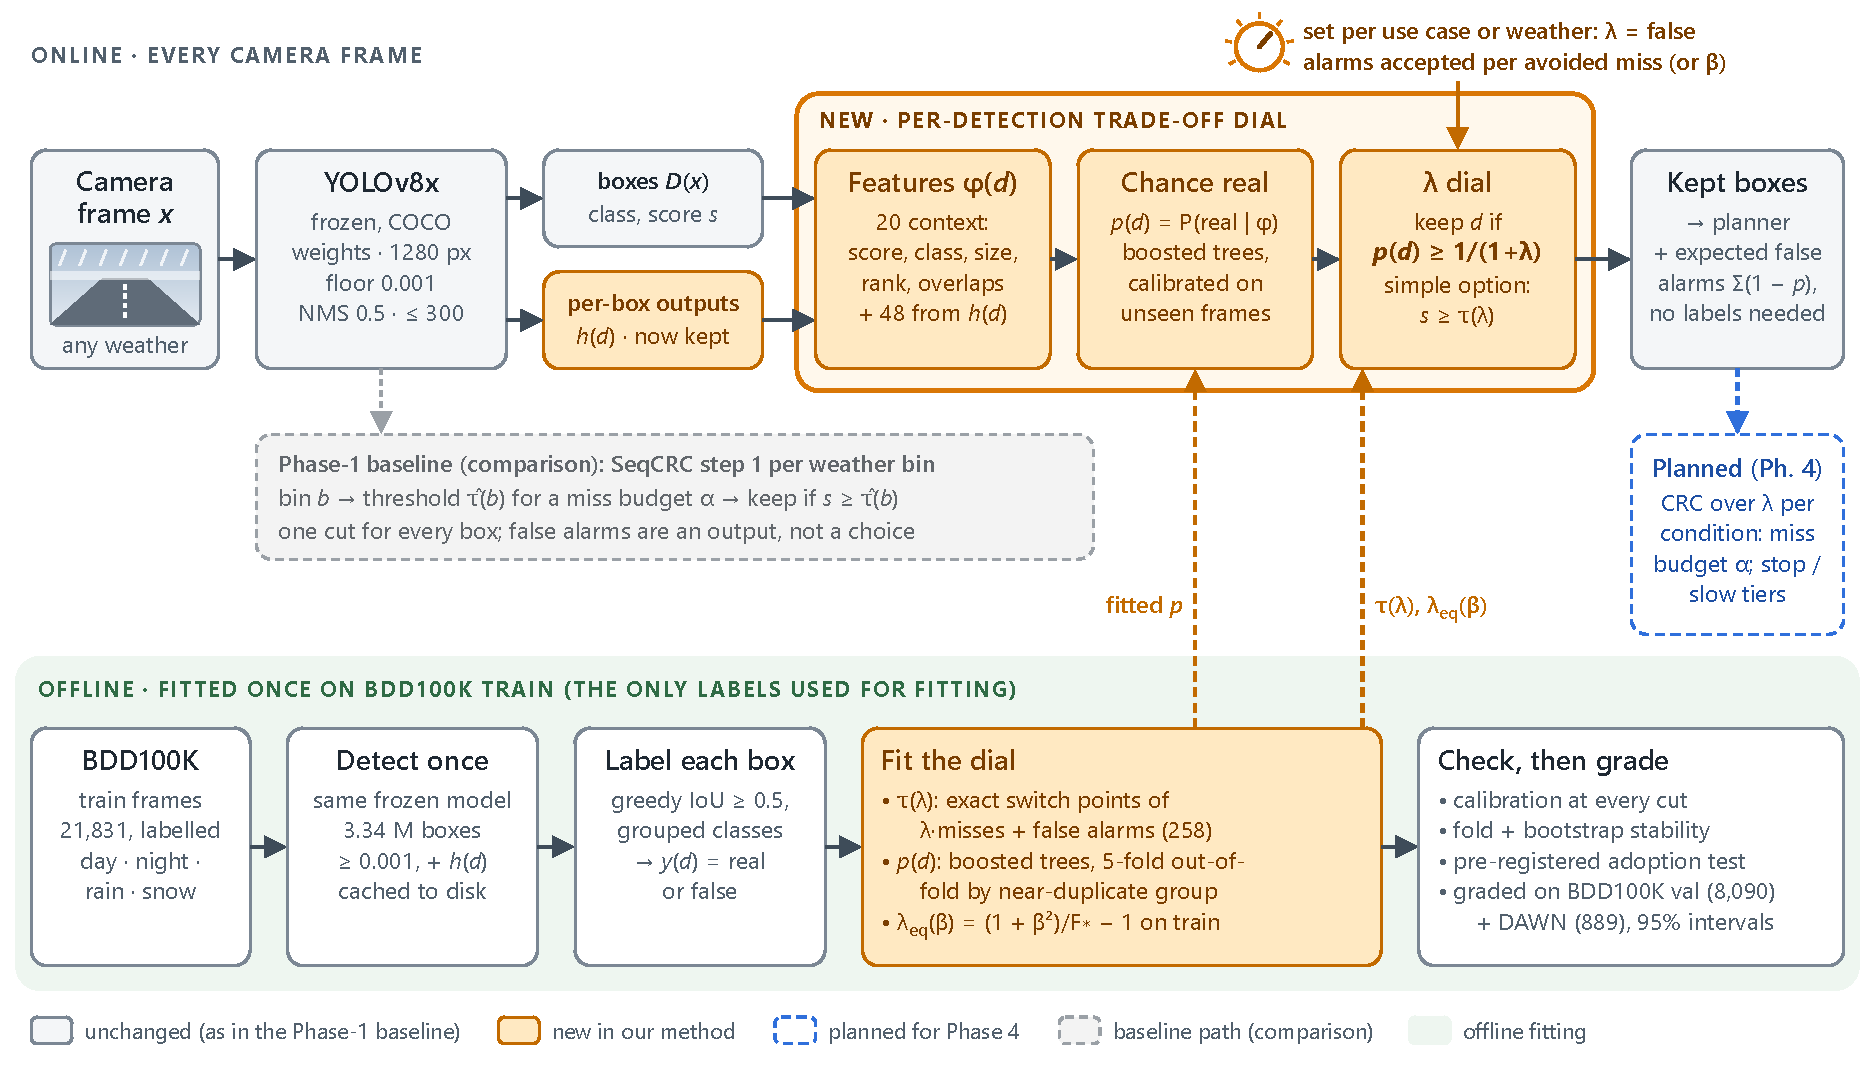
\includegraphics[width=\textwidth]{architecture}
  \caption{Architecture. New components are orange, unchanged ones grey; the dashed grey lane is the Phase-1
  baseline, kept for comparison, and the dashed blue box is planned for Phase~4. Fitting (green band) uses only
  BDD100K train; grading uses BDD100K val and DAWN.}
  \label{fig:architecture}
\end{figure}

\subsection{Algorithm}\label{sec:method-alg}

\paragraph{Cost.} For a keep rule $k$ over the detections of image $x$, let $M_k(x)$ be the number of
ground-truth objects left without a kept matched box and $F_k(x)$ the number of kept boxes that match no object.
The dial setting $\lambda > 0$ defines the cost
\begin{equation}
  C_\lambda(k) \;=\; \sum_{x}\big[\lambda\, M_k(x) + F_k(x)\big].
  \label{eq:cost}
\end{equation}

\paragraph{Option A: one threshold.} $k(d) = \mathbf{1}[s(d) \ge \tau(\lambda)]$ with
\begin{equation}
  \tau(\lambda) \;=\; \arg\min_{\tau} \sum_{x \in \mathcal{D}_{\text{train}}} \big[\lambda\, M_\tau(x) + F_\tau(x)\big].
  \label{eq:one-threshold}
\end{equation}
Greedy non-maximum suppression and greedy matching are both score-ordered, so filtering one detector run at
$\tau$ equals running the detector at $\tau$. Equation~\eqref{eq:one-threshold} is therefore solved exactly from
cumulative counts: the minimisers for all $\lambda$ are the corners of the lower convex hull of
(real kept, false kept), stored as 258 switch points.

\paragraph{Option B: per detection.} Keeping a box with probability $p$ of being real costs an expected
$1-p$ false alarms; dropping it costs an expected $\lambda p$ in misses. The cost-optimal rule is
therefore~\citep{elkan2001foundations}
\begin{equation}
  \text{keep } d \iff 1 - p(d) \le \lambda\, p(d) \iff p(d) \ge \frac{1}{1+\lambda},
  \label{eq:bayes}
\end{equation}
which is optimal when $p$ is calibrated. Because the kept set grows with $\lambda$, the miss count is
non-increasing in $\lambda$. We estimate $p(d) = \sigma\big(g(\varphi(d))\big)$ with gradient-boosted
trees~\citep{friedman2001gbm,ke2017lightgbm,pedregosa2011sklearn}. They are trained on all train detections by
minimising the log-loss
$\ell = -\sum_d \big[y_d \log p_d + (1-y_d)\log(1-p_d)\big]$, where $y_d \in \{0,1\}$ comes from greedy
IoU-$0.5$ matching with grouped classes (vehicle, two-wheeler, person). We check calibration with the expected
calibration error~\citep{guo2017calibration} and with the share of real boxes among detections near each cut
$1/(1+\lambda)$.

\paragraph{F-score units.} With calibrated probabilities, the $F_\beta$-optimal cut is $F^*_\beta/(1+\beta^2)$,
where $F^*_\beta$ is the best achievable $F_\beta$~\citep{zhao2013beyond,lipton2014optimal}. Setting this cut
equal to $1/(1+\lambda)$ gives the equivalent dial setting
\begin{equation}
  \lambda_{\text{eq}}(\beta) \;=\; \frac{1+\beta^2}{F^*_\beta} - 1,
  \label{eq:fbeta}
\end{equation}
with $F^*_\beta$ measured on train for each option. For example, $F_1$ corresponds to $\lambda \approx 1.8$ and
$F_2$ to $\lambda \approx 6.2$ with the per-detection option.

\paragraph{Planned: a miss budget on top of the dial (CRC over $\lambda$).} Because the image-level miss fraction
$L_i(\lambda)$ is non-increasing in $\lambda$, the baseline's rule~\eqref{eq:baseline-crc} applies to $\lambda$
itself. Per condition $c$ with $n_c$ calibration images,
\begin{equation}
  \hat\lambda_c \;=\; \inf\Big\{\lambda \;:\; \tfrac{n_c}{n_c+1}\,\hat R_c(\lambda) + \tfrac{1}{n_c+1} \le \alpha\Big\},
  \label{eq:crc-lambda}
\end{equation}
and deploying $\max(\lambda_{\text{user}}, \hat\lambda_c)$ keeps the CRC guarantee
$\mathbb{E}[L_{\text{test}}] \le \alpha$ under exchangeability within the condition, while never being less
cautious than the user asked. The fit is infeasible when $\alpha$ is below the miss fraction at the score floor
(11--18\% of objects are never detected).

\begin{algorithm}[t]
\caption{Fitting the dial (offline, BDD100K train only)}\label{alg:fit}
\begin{algorithmic}[1]
\Require labelled train frames $\mathcal{D}_{\text{train}}$; frozen detector $f$
\ForAll{$x \in \mathcal{D}_{\text{train}}$}
  \State $(D(x), h) \gets f(x)$ \Comment{floor 0.001, NMS 0.5, $\le 300$ boxes; keep per-box outputs}
  \State $y(d) \gets$ greedy IoU $\ge 0.5$ match of $d \in D(x)$ to labels \Comment{grouped classes}
\EndFor
\State \textbf{Option A:} sort scores; keep ends of equal-score blocks; cumulative real and false counts
\State \hspace{1.2em} $\tau(\cdot) \gets$ corners of the lower convex hull \Comment{all $\lambda$ at once}
\State \textbf{Option B:} $\varphi(d) \gets [\text{context}(d, D(x)),\ \text{per-box}(h(d))]$ \Comment{PCA fitted on train}
\State \hspace{1.2em} $g \gets$ gradient boosting on $\{(\varphi(d), y(d))\}$ \Comment{log-loss}
\State \hspace{1.2em} $p_{\text{oof}} \gets$ 5-fold out-of-fold probabilities, folds by near-duplicate group
\ForAll{$\beta$}
  \State $\lambda_{\text{eq}}(\beta) \gets (1+\beta^2)/F^*_\beta - 1$ \Comment{F-score map, $F^*_\beta$ on train}
\EndFor
\State check calibration near every cut $1/(1+\lambda)$ and fold stability; adopt only if the pre-registered criteria hold
\State \Return $\tau(\cdot)$, $g$ (with PCA), $\lambda_{\text{eq}}(\cdot)$
\end{algorithmic}
\end{algorithm}

\begin{algorithm}[t]
\caption{Applying the dial (online, every camera frame)}\label{alg:deploy}
\begin{algorithmic}[1]
\Require frame $x$; setting $\lambda$ (or $\beta$); option $\in\{$A, B$\}$
\If{$\beta$ is given} \State $\lambda \gets \lambda_{\text{eq}}(\beta)$ \Comment{F-score map} \EndIf
\If{a budget $\alpha$ is certified for condition $c$} \State $\lambda \gets \max(\lambda, \hat\lambda_c)$ \Comment{planned: CRC over $\lambda$} \EndIf
\State $(D, h) \gets f(x)$ \Comment{one detector pass}
\ForAll{$d \in D$}
  \If{option A}
    \State keep $d$ iff $s(d) \ge \tau(\lambda)$
  \Else
    \State $p(d) \gets \sigma(g(\varphi(d)))$; keep $d$ iff $p(d) \ge 1/(1+\lambda)$ \Comment{cost-optimal cut}
  \EndIf
\EndFor
\State $\widehat{\mathrm{FA}} \gets \sum_{d \text{ kept}} (1 - p(d))$ \Comment{expected false alarms, no labels needed}
\State \Return kept detections, $\widehat{\mathrm{FA}}$
\end{algorithmic}
\end{algorithm}

\subsection{Design choices}\label{sec:method-design}

Table~\ref{tab:design} gives each design choice, the reason for it, and the alternatives we tried or
considered. Most of the alternatives were run in the harness, several under pre-registered criteria.

\begin{table}[t]
\centering\small
\caption{Design choices, the reasons for them, and the alternatives considered (with the evidence).}
\label{tab:design}
\begin{tabularx}{\textwidth}{@{}>{\raggedright\arraybackslash}p{2.9cm}>{\raggedright\arraybackslash}X>{\raggedright\arraybackslash}X@{}}
\toprule
Choice & Why & Alternatives considered \\
\midrule
Keep the detector frozen; decide after it &
calibration stays valid; one detector run serves every setting; no retraining per condition &
domain adaptation (DA-Detect: 20.41 vs 21.44 AP@50 on real DAWN fog in Phase~1); fine-tuning (invalidates every calibration) \\
Trade-off as $\lambda$, false alarms per avoided miss &
use case sets the balance; the optimal rule is explicit (Eq.~\ref{eq:bayes}); $\beta$ and $\alpha$ map onto it &
fixed $\alpha$ only (baseline, false alarms unpriced); maximise $F_1$ (one fixed balance); FPPI cap \\
Decide per detection &
87--91\% of a per-image oracle's advantage on BDD100K is chance; the learnable signal is in individual boxes &
per-image thresholds from pixels, from the confidence profile, or from YOLOv8x image features (all failed pre-registered tests); box-combination rules; summed-confidence maps \\
One threshold kept as the simple option &
one auditable number per $\lambda$; per-weather thresholds give no gain (0.98--1.03$\times$ the cost) &
per-weather thresholds (the baseline's form) \\
Gradient-boosted trees on detector outputs &
tabular inputs; trains in minutes on CPU; calibrated without post-hoc scaling (expected calibration error 0.11 points on BDD100K val) &
recalibrating the score alone (this is Option~A); a neural head; retraining YOLOv8x's head \\
YOLOv8x's own per-box outputs as features &
pre-registered gain: cost 0.972$\times$ (0.969--0.975) of the context-only model on BDD100K, not worse on DAWN (0.995) &
context features only (model~1); a separate CNN on box crops (more compute) \\
One model for every $\beta$ &
theory: only the cut moves with $\beta$; dedicated $\beta$-weighted models tie (0.997--1.001$\times$) &
one cost-weighted model per $\beta$ \\
Fit on BDD100K train; grade on BDD100K val and DAWN &
nothing is chosen on graded data; DAWN tests transfer to real fog, rain, sand and snow &
calibrating on halves of the test pool (the baseline protocol) \\
Grouped classes in matching &
car/truck confusions are not safety misses &
class-aware matching (run~1) \\
\bottomrule
\end{tabularx}
\end{table}

\subsection{Experiment plan (Phase~4)}\label{sec:method-plan}

\paragraph{Data and splits.} The dial is fitted on 21,831 BDD100K train frames (3.34\,M detections), with 5-fold
out-of-fold estimates grouped by near-duplicate group. It is graded on BDD100K val (8,090 frames in seven
weather-by-time bins) and on DAWN (889 frames with clean labels: fog 256, rain 187, sand 243, snow 203).
Neither set is used for any choice. For CRC over $\lambda$ we use 200 random calibration/test halves per
condition, keeping near-duplicate groups together, as in the baseline runs.

\paragraph{Metrics.} The main metric is the cost $C_\lambda$ relative to one threshold, with 95\% image-bootstrap
intervals~\citep{efron1993bootstrap}. We also report recall, precision and false alarms per image at
$\lambda \in \{1, 3, 10, 30, 100\}$; $F_\beta$ at $\beta \in \{0.5, 1, 2\}$ against no tuning and the best
in-sample constant; and calibration (expected calibration error, share real near each cut). For CRC over
$\lambda$ we report the held-out miss fraction against $\alpha$ (share of splits above), its price in false alarms
per image, and the smallest certifiable $\alpha$.

\paragraph{Baselines.} (i) No tuning ($\tau = 0.25$, the Ultralytics default). (ii) One global CRC threshold.
(iii) The per-weather CRC threshold, Eq.~\eqref{eq:baseline-crc} (Phase-1 baseline). (iv) Option~A, the one-threshold
dial. (v) The context-only per-detection model. As reference bounds that no deployable rule can reach, we also
report the best constant threshold chosen in-sample per condition and the per-frame hindsight best.

\paragraph{Ablations.} (a) Retraining without each feature group: class probabilities, neck components, DFL
entropy, level, context. (b) Per-condition recalibration, which targets the under-stated probabilities in DAWN fog
(17\% real at the 9.1\% cut). (c) Training-set size: 25, 50 and 100\% of frames. (d) Detector size and input
resolution: YOLOv8x at 640 versus 1280, and YOLOv8s. (e) CRC over $\lambda$ versus CRC over $\tau$ at equal
$\alpha$. Already completed: model~1 versus model~2, per-weather thresholds, and dedicated $\beta$ models.

\paragraph{Compute.} Measured on our laptop GPU (RTX 3050 Ti, 4\,GB):
\begin{itemize}
  \item YOLOv8x at 1280\,px takes 0.15--0.17\,s per frame;
  \item extracting per-box outputs for all 30.9k frames takes about 85 minutes;
  \item fitting the per-detection model takes about 11 minutes on the CPU;
  \item the CRC splits take minutes on the CPU.
\end{itemize}
We will use an NRP A100 for the new detector passes in ablation~(d) and for the repeated fits in (a)--(c).
At an estimated $\ge 10\times$ the laptop's throughput, these take a few GPU-hours in total. The laptop
remains a fallback for every step.
. Needs the lit-review preamble plus:
%   \usepackage{algorithm}  \usepackage{algpseudocode}          (see preamble_additions.tex)
% Figure: upload ../figures/phase3/architecture.pdf (same drawing as architecture.svg on the slides).
% Citations: keys from refs_litreview.bib plus refs_methodology.bib.
% Every number is from the harness result files; see Docs/08_method_lambda_dial.md and Docs/05_results_crc_runs.md.
% ============================================================================================================
\section{Methodology}\label{sec:method}

\subsection{Baseline: per-weather conformal threshold (Phase~1)}\label{sec:method-baseline}

Our baseline is the first step of SeqCRC~\citep{andeol2025seqcrc}: conformal risk control
(CRC)~\citep{angelopoulos2024crc} on the confidence threshold of a frozen detector, with an image-level loss
$L_i(\tau)$, the fraction of ground-truth objects in calibration image~$i$ with no matched detection scoring at
least~$\tau$. Calibrated separately in each weather bin~$b$ with $n$ calibration images, the threshold is
\begin{equation}
  \hat\tau(b) \;=\; \max\Big\{\tau \;:\; \tfrac{n}{n+1}\,\hat R(\tau; b) + \tfrac{1}{n+1} \le \alpha\Big\},
  \qquad \hat R(\tau; b) = \tfrac{1}{n}\textstyle\sum_{i=1}^{n} L_i(\tau),
  \label{eq:baseline-crc}
\end{equation}
which bounds the expected miss fraction of an exchangeable test image from the same bin by~$\alpha$.
In Phase~1 we reproduced SeqCRC with its official code (the guarantee held in 5 of 5 configurations on COCO)
and ran it on DAWN~\citep{kenk2020dawn}. Our harness implements Eq.~\eqref{eq:baseline-crc} per weather bin on
YOLOv8x~\citep{ultralytics2023yolov8}. With $\alpha = 0.2$ on DAWN, the per-bin threshold keeps the held-out miss
fraction at 0.188--0.194 in every bin, at 1.6--6.2 false positives per image (FPPI), while one global threshold
misses 0.251 in fog (above $\alpha$ in 98\% of 200 splits). On BDD100K~\citep{yu2020bdd100k}, a threshold
calibrated on clear days misses 0.28--0.36 at night; per-bin thresholds restore the budget at 43--117 FPPI.

\paragraph{Limitation (the gap).} The baseline fixes the miss budget and lets the false alarms be whatever
results: at night it buys $\alpha = 0.2$ with up to 117 false alarms per image, and there is no way to ask for a
different balance. It applies one score cut to every box, it needs the weather bin at run time (our camera-only
weather estimators did not isolate fog), and its guarantee assumes exchangeable data within each bin.

\subsection{Proposed method: a calibrated trade-off dial}\label{sec:method-idea}

\textbf{Core idea.} Instead of one confidence threshold per weather bin, every detection receives a calibrated
probability $p(d)$ that it is a real object, computed from the frozen detector's own outputs, and is kept if and
only if $p(d) \ge 1/(1+\lambda)$. The single user-facing parameter $\lambda$, the number of false alarms
accepted to avoid one missed object, sets the trade-off for the use case. An F-score weight $\beta$ (and, in
Phase~4, a CRC miss budget $\alpha$) maps onto the same dial.

Table~\ref{tab:changes} lists what changes relative to the baseline. The detector, data, matching rule and
evaluation protocol stay the same; only the decision of which boxes to keep is replaced.

\begin{table}[t]
\centering\small
\caption{What our method keeps, replaces and adds relative to the Phase-1 baseline.}
\label{tab:changes}
\begin{tabularx}{\textwidth}{@{}>{\raggedright\arraybackslash}p{2.6cm}>{\raggedright\arraybackslash}X>{\raggedright\arraybackslash}X@{}}
\toprule
 & Baseline (SeqCRC step~1 per weather bin) & Ours (trade-off dial) \\
\midrule
Detector & YOLOv8x, frozen COCO weights, 1280\,px, score floor 0.001 & unchanged \\
Decision rule & one score threshold per weather bin, $s \ge \hat\tau(b)$ & per detection, $p(d) \ge 1/(1+\lambda)$; simple option: one threshold $s \ge \tau(\lambda)$ \\
Trade-off & fixed miss budget $\alpha$; false alarms unpriced & explicit input $\lambda$ (or $\beta$); $\alpha$ planned as a floor via CRC over $\lambda$ \\
Run-time inputs & score and the weather bin & score, box context and the detector's per-box outputs (no weather label) \\
Fitting & calibration half of each bin & once, on 21,831 labelled BDD100K train frames \\
Added & --- & per-box feature tap; calibrated model; $\beta \to \lambda$ map; label-free estimate of false alarms \\
\bottomrule
\end{tabularx}
\end{table}

\subsection{Architecture}\label{sec:method-arch}

Figure~\ref{fig:architecture} shows the full pipeline. Online, YOLOv8x runs once per camera frame and returns
candidate boxes $D(x)$ with class and score~$s$. We also keep the detector's per-box outputs $h(d)$ at the
anchor each box came from: the 80 class probabilities, the four distribution-focal-loss (DFL) distributions over
the box sides~\citep{li2020gfl}, the neck feature vector, and the pyramid level. A feature builder forms
$\varphi(d)$: 20 context features (score, class, size and position, rank, overlap with stronger boxes, crowding)
plus 48 per-box features (six class probabilities, strongest other class, top-two margin, sum and entropy of the
probabilities, DFL entropy per side and mean, level, and 32 principal components of the neck feature).
A gradient-boosted model maps $\varphi(d)$ to $p(d)$, and the dial keeps or drops each box. Offline, the same
frozen detector is run once over BDD100K train, boxes are labelled by matching, and the dial is fitted, checked
and then graded on data never used for fitting.

\begin{figure}[t]
  \centering
  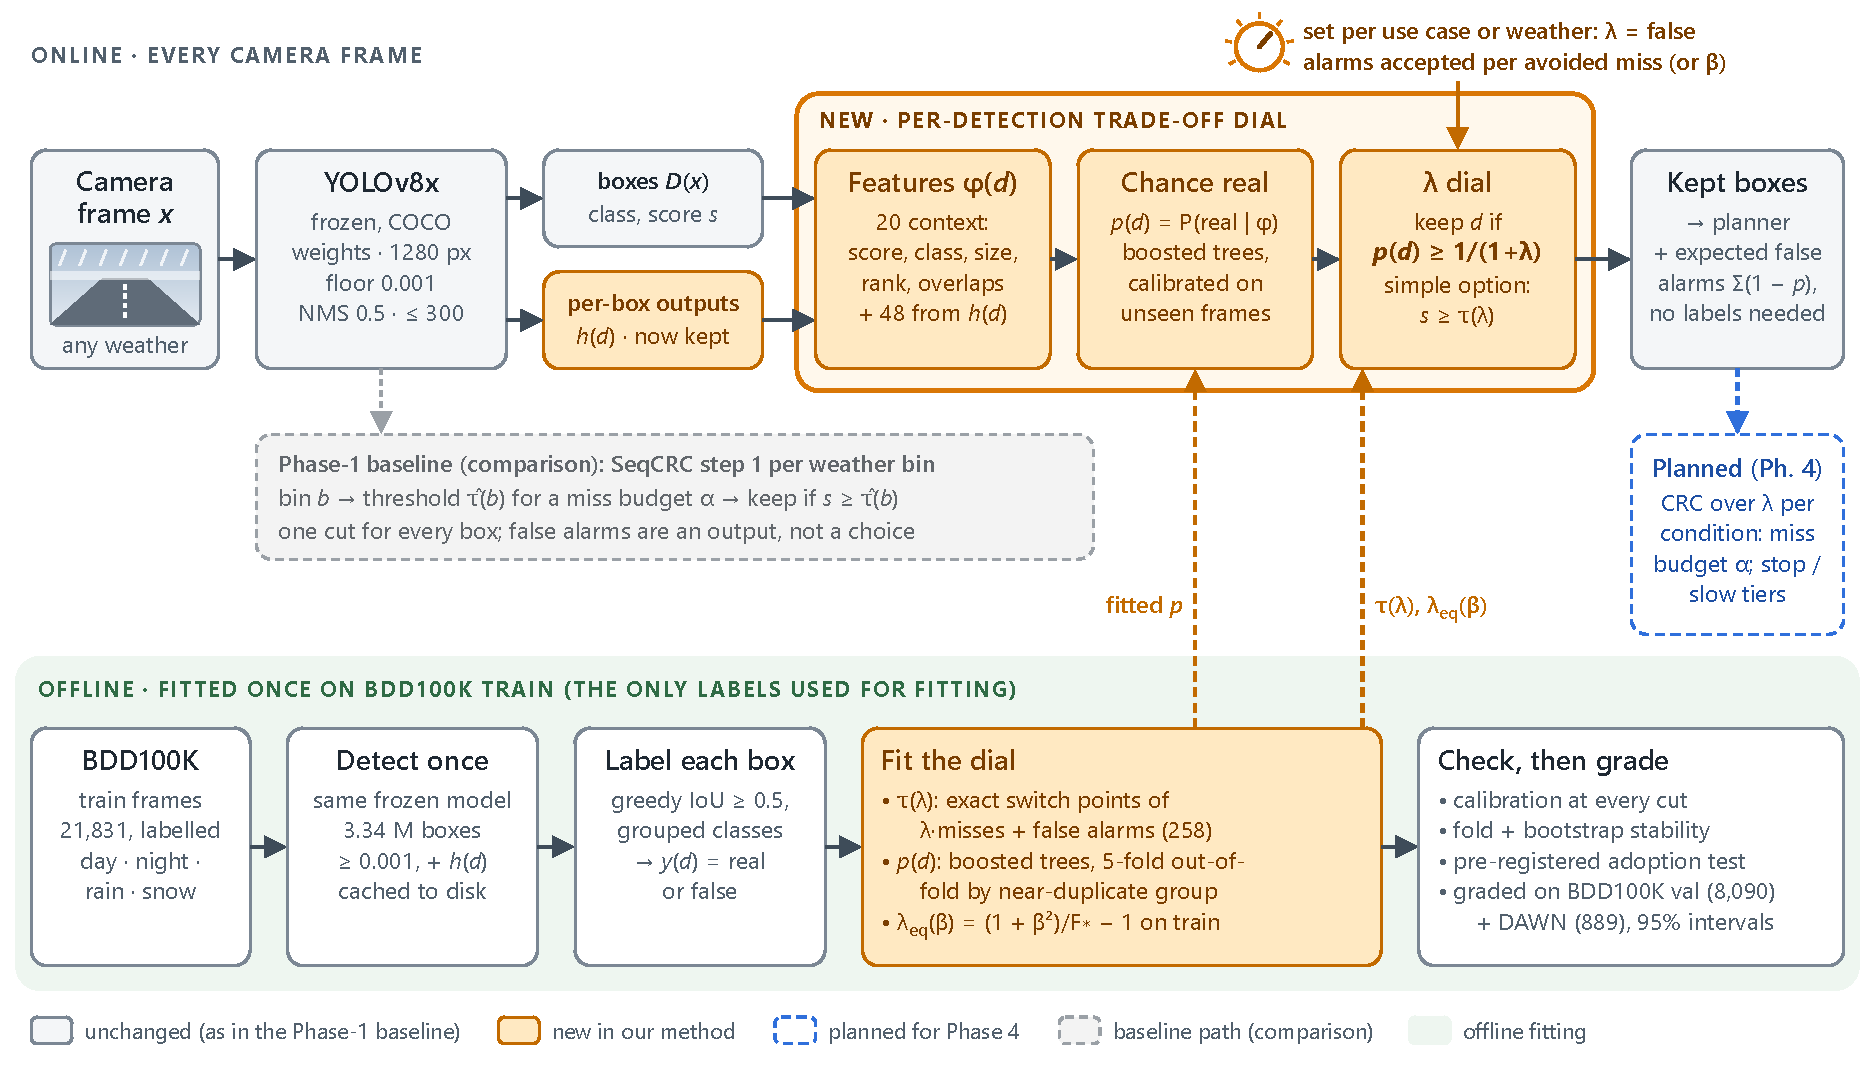
\includegraphics[width=\textwidth]{architecture}
  \caption{Architecture. New components are orange, unchanged ones grey; the dashed grey lane is the Phase-1
  baseline, kept for comparison, and the dashed blue box is planned for Phase~4. Fitting (green band) uses only
  BDD100K train; grading uses BDD100K val and DAWN.}
  \label{fig:architecture}
\end{figure}

\subsection{Algorithm}\label{sec:method-alg}

\paragraph{Cost.} For a keep rule $k$ over the detections of image $x$, let $M_k(x)$ be the number of
ground-truth objects left without a kept matched box and $F_k(x)$ the number of kept boxes that match no object.
The dial setting $\lambda > 0$ defines the cost
\begin{equation}
  C_\lambda(k) \;=\; \sum_{x}\big[\lambda\, M_k(x) + F_k(x)\big].
  \label{eq:cost}
\end{equation}

\paragraph{Option A: one threshold.} $k(d) = \mathbf{1}[s(d) \ge \tau(\lambda)]$ with
\begin{equation}
  \tau(\lambda) \;=\; \arg\min_{\tau} \sum_{x \in \mathcal{D}_{\text{train}}} \big[\lambda\, M_\tau(x) + F_\tau(x)\big].
  \label{eq:one-threshold}
\end{equation}
Greedy non-maximum suppression and greedy matching are both score-ordered, so filtering one detector run at
$\tau$ equals running the detector at $\tau$. Equation~\eqref{eq:one-threshold} is therefore solved exactly from
cumulative counts: the minimisers for all $\lambda$ are the corners of the lower convex hull of
(real kept, false kept), stored as 258 switch points.

\paragraph{Option B: per detection.} Keeping a box with probability $p$ of being real costs an expected
$1-p$ false alarms; dropping it costs an expected $\lambda p$ in misses. The cost-optimal rule is
therefore~\citep{elkan2001foundations}
\begin{equation}
  \text{keep } d \iff 1 - p(d) \le \lambda\, p(d) \iff p(d) \ge \frac{1}{1+\lambda},
  \label{eq:bayes}
\end{equation}
which is optimal when $p$ is calibrated. Because the kept set grows with $\lambda$, the miss count is
non-increasing in $\lambda$. We estimate $p(d) = \sigma\big(g(\varphi(d))\big)$ with gradient-boosted
trees~\citep{friedman2001gbm,ke2017lightgbm,pedregosa2011sklearn}. They are trained on all train detections by
minimising the log-loss
$\ell = -\sum_d \big[y_d \log p_d + (1-y_d)\log(1-p_d)\big]$, where $y_d \in \{0,1\}$ comes from greedy
IoU-$0.5$ matching with grouped classes (vehicle, two-wheeler, person). We check calibration with the expected
calibration error~\citep{guo2017calibration} and with the share of real boxes among detections near each cut
$1/(1+\lambda)$.

\paragraph{F-score units.} With calibrated probabilities, the $F_\beta$-optimal cut is $F^*_\beta/(1+\beta^2)$,
where $F^*_\beta$ is the best achievable $F_\beta$~\citep{zhao2013beyond,lipton2014optimal}. Setting this cut
equal to $1/(1+\lambda)$ gives the equivalent dial setting
\begin{equation}
  \lambda_{\text{eq}}(\beta) \;=\; \frac{1+\beta^2}{F^*_\beta} - 1,
  \label{eq:fbeta}
\end{equation}
with $F^*_\beta$ measured on train for each option. For example, $F_1$ corresponds to $\lambda \approx 1.8$ and
$F_2$ to $\lambda \approx 6.2$ with the per-detection option.

\paragraph{Planned: a miss budget on top of the dial (CRC over $\lambda$).} Because the image-level miss fraction
$L_i(\lambda)$ is non-increasing in $\lambda$, the baseline's rule~\eqref{eq:baseline-crc} applies to $\lambda$
itself. Per condition $c$ with $n_c$ calibration images,
\begin{equation}
  \hat\lambda_c \;=\; \inf\Big\{\lambda \;:\; \tfrac{n_c}{n_c+1}\,\hat R_c(\lambda) + \tfrac{1}{n_c+1} \le \alpha\Big\},
  \label{eq:crc-lambda}
\end{equation}
and deploying $\max(\lambda_{\text{user}}, \hat\lambda_c)$ keeps the CRC guarantee
$\mathbb{E}[L_{\text{test}}] \le \alpha$ under exchangeability within the condition, while never being less
cautious than the user asked. The fit is infeasible when $\alpha$ is below the miss fraction at the score floor
(11--18\% of objects are never detected).

\begin{algorithm}[t]
\caption{Fitting the dial (offline, BDD100K train only)}\label{alg:fit}
\begin{algorithmic}[1]
\Require labelled train frames $\mathcal{D}_{\text{train}}$; frozen detector $f$
\ForAll{$x \in \mathcal{D}_{\text{train}}$}
  \State $(D(x), h) \gets f(x)$ \Comment{floor 0.001, NMS 0.5, $\le 300$ boxes; keep per-box outputs}
  \State $y(d) \gets$ greedy IoU $\ge 0.5$ match of $d \in D(x)$ to labels \Comment{grouped classes}
\EndFor
\State \textbf{Option A:} sort scores; keep ends of equal-score blocks; cumulative real and false counts
\State \hspace{1.2em} $\tau(\cdot) \gets$ corners of the lower convex hull \Comment{all $\lambda$ at once}
\State \textbf{Option B:} $\varphi(d) \gets [\text{context}(d, D(x)),\ \text{per-box}(h(d))]$ \Comment{PCA fitted on train}
\State \hspace{1.2em} $g \gets$ gradient boosting on $\{(\varphi(d), y(d))\}$ \Comment{log-loss}
\State \hspace{1.2em} $p_{\text{oof}} \gets$ 5-fold out-of-fold probabilities, folds by near-duplicate group
\ForAll{$\beta$}
  \State $\lambda_{\text{eq}}(\beta) \gets (1+\beta^2)/F^*_\beta - 1$ \Comment{F-score map, $F^*_\beta$ on train}
\EndFor
\State check calibration near every cut $1/(1+\lambda)$ and fold stability; adopt only if the pre-registered criteria hold
\State \Return $\tau(\cdot)$, $g$ (with PCA), $\lambda_{\text{eq}}(\cdot)$
\end{algorithmic}
\end{algorithm}

\begin{algorithm}[t]
\caption{Applying the dial (online, every camera frame)}\label{alg:deploy}
\begin{algorithmic}[1]
\Require frame $x$; setting $\lambda$ (or $\beta$); option $\in\{$A, B$\}$
\If{$\beta$ is given} \State $\lambda \gets \lambda_{\text{eq}}(\beta)$ \Comment{F-score map} \EndIf
\If{a budget $\alpha$ is certified for condition $c$} \State $\lambda \gets \max(\lambda, \hat\lambda_c)$ \Comment{planned: CRC over $\lambda$} \EndIf
\State $(D, h) \gets f(x)$ \Comment{one detector pass}
\ForAll{$d \in D$}
  \If{option A}
    \State keep $d$ iff $s(d) \ge \tau(\lambda)$
  \Else
    \State $p(d) \gets \sigma(g(\varphi(d)))$; keep $d$ iff $p(d) \ge 1/(1+\lambda)$ \Comment{cost-optimal cut}
  \EndIf
\EndFor
\State $\widehat{\mathrm{FA}} \gets \sum_{d \text{ kept}} (1 - p(d))$ \Comment{expected false alarms, no labels needed}
\State \Return kept detections, $\widehat{\mathrm{FA}}$
\end{algorithmic}
\end{algorithm}

\subsection{Design choices}\label{sec:method-design}

Table~\ref{tab:design} gives each design choice, the reason for it, and the alternatives we tried or
considered. Most of the alternatives were run in the harness, several under pre-registered criteria.

\begin{table}[t]
\centering\small
\caption{Design choices, the reasons for them, and the alternatives considered (with the evidence).}
\label{tab:design}
\begin{tabularx}{\textwidth}{@{}>{\raggedright\arraybackslash}p{2.9cm}>{\raggedright\arraybackslash}X>{\raggedright\arraybackslash}X@{}}
\toprule
Choice & Why & Alternatives considered \\
\midrule
Keep the detector frozen; decide after it &
calibration stays valid; one detector run serves every setting; no retraining per condition &
domain adaptation (DA-Detect: 20.41 vs 21.44 AP@50 on real DAWN fog in Phase~1); fine-tuning (invalidates every calibration) \\
Trade-off as $\lambda$, false alarms per avoided miss &
use case sets the balance; the optimal rule is explicit (Eq.~\ref{eq:bayes}); $\beta$ and $\alpha$ map onto it &
fixed $\alpha$ only (baseline, false alarms unpriced); maximise $F_1$ (one fixed balance); FPPI cap \\
Decide per detection &
87--91\% of a per-image oracle's advantage on BDD100K is chance; the learnable signal is in individual boxes &
per-image thresholds from pixels, from the confidence profile, or from YOLOv8x image features (all failed pre-registered tests); box-combination rules; summed-confidence maps \\
One threshold kept as the simple option &
one auditable number per $\lambda$; per-weather thresholds give no gain (0.98--1.03$\times$ the cost) &
per-weather thresholds (the baseline's form) \\
Gradient-boosted trees on detector outputs &
tabular inputs; trains in minutes on CPU; calibrated without post-hoc scaling (expected calibration error 0.11 points on BDD100K val) &
recalibrating the score alone (this is Option~A); a neural head; retraining YOLOv8x's head \\
YOLOv8x's own per-box outputs as features &
pre-registered gain: cost 0.972$\times$ (0.969--0.975) of the context-only model on BDD100K, not worse on DAWN (0.995) &
context features only (model~1); a separate CNN on box crops (more compute) \\
One model for every $\beta$ &
theory: only the cut moves with $\beta$; dedicated $\beta$-weighted models tie (0.997--1.001$\times$) &
one cost-weighted model per $\beta$ \\
Fit on BDD100K train; grade on BDD100K val and DAWN &
nothing is chosen on graded data; DAWN tests transfer to real fog, rain, sand and snow &
calibrating on halves of the test pool (the baseline protocol) \\
Grouped classes in matching &
car/truck confusions are not safety misses &
class-aware matching (run~1) \\
\bottomrule
\end{tabularx}
\end{table}

\subsection{Experiment plan (Phase~4)}\label{sec:method-plan}

\paragraph{Data and splits.} The dial is fitted on 21,831 BDD100K train frames (3.34\,M detections), with 5-fold
out-of-fold estimates grouped by near-duplicate group. It is graded on BDD100K val (8,090 frames in seven
weather-by-time bins) and on DAWN (889 frames with clean labels: fog 256, rain 187, sand 243, snow 203).
Neither set is used for any choice. For CRC over $\lambda$ we use 200 random calibration/test halves per
condition, keeping near-duplicate groups together, as in the baseline runs.

\paragraph{Metrics.} The main metric is the cost $C_\lambda$ relative to one threshold, with 95\% image-bootstrap
intervals~\citep{efron1993bootstrap}. We also report recall, precision and false alarms per image at
$\lambda \in \{1, 3, 10, 30, 100\}$; $F_\beta$ at $\beta \in \{0.5, 1, 2\}$ against no tuning and the best
in-sample constant; and calibration (expected calibration error, share real near each cut). For CRC over
$\lambda$ we report the held-out miss fraction against $\alpha$ (share of splits above), its price in false alarms
per image, and the smallest certifiable $\alpha$.

\paragraph{Baselines.} (i) No tuning ($\tau = 0.25$, the Ultralytics default). (ii) One global CRC threshold.
(iii) The per-weather CRC threshold, Eq.~\eqref{eq:baseline-crc} (Phase-1 baseline). (iv) Option~A, the one-threshold
dial. (v) The context-only per-detection model. As reference bounds that no deployable rule can reach, we also
report the best constant threshold chosen in-sample per condition and the per-frame hindsight best.

\paragraph{Ablations.} (a) Retraining without each feature group: class probabilities, neck components, DFL
entropy, level, context. (b) Per-condition recalibration, which targets the under-stated probabilities in DAWN fog
(17\% real at the 9.1\% cut). (c) Training-set size: 25, 50 and 100\% of frames. (d) Detector size and input
resolution: YOLOv8x at 640 versus 1280, and YOLOv8s. (e) CRC over $\lambda$ versus CRC over $\tau$ at equal
$\alpha$. Already completed: model~1 versus model~2, per-weather thresholds, and dedicated $\beta$ models.

\paragraph{Compute.} Measured on our laptop GPU (RTX 3050 Ti, 4\,GB):
\begin{itemize}
  \item YOLOv8x at 1280\,px takes 0.15--0.17\,s per frame;
  \item extracting per-box outputs for all 30.9k frames takes about 85 minutes;
  \item fitting the per-detection model takes about 11 minutes on the CPU;
  \item the CRC splits take minutes on the CPU.
\end{itemize}
We will use an NRP A100 for the new detector passes in ablation~(d) and for the repeated fits in (a)--(c).
At an estimated $\ge 10\times$ the laptop's throughput, these take a few GPU-hours in total. The laptop
remains a fallback for every step.
